%%-*- mode: LaTeX; mode: FlySpell; -*-

\section{Abstraction over events}
\label{sec:event}

\begin{figure*}
	\centering
	%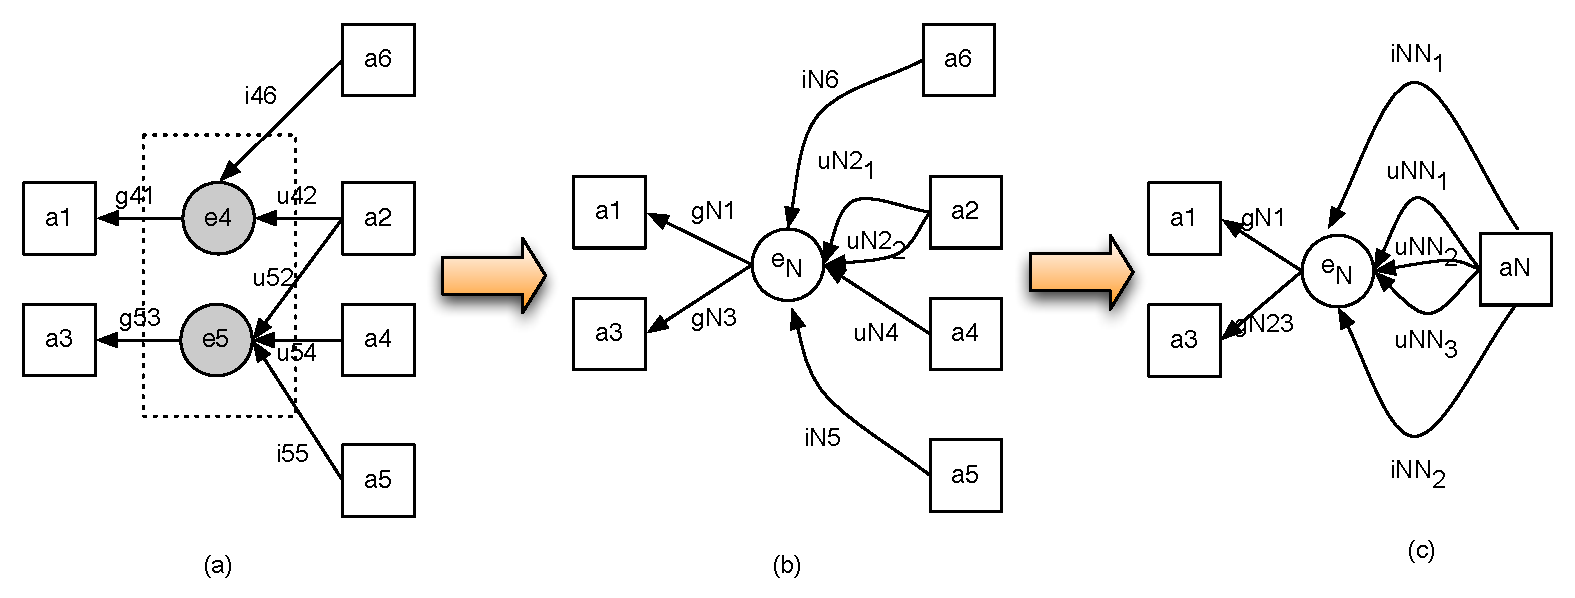
\includegraphics[scale=.5]{figures/e4-e5.pdf} 
	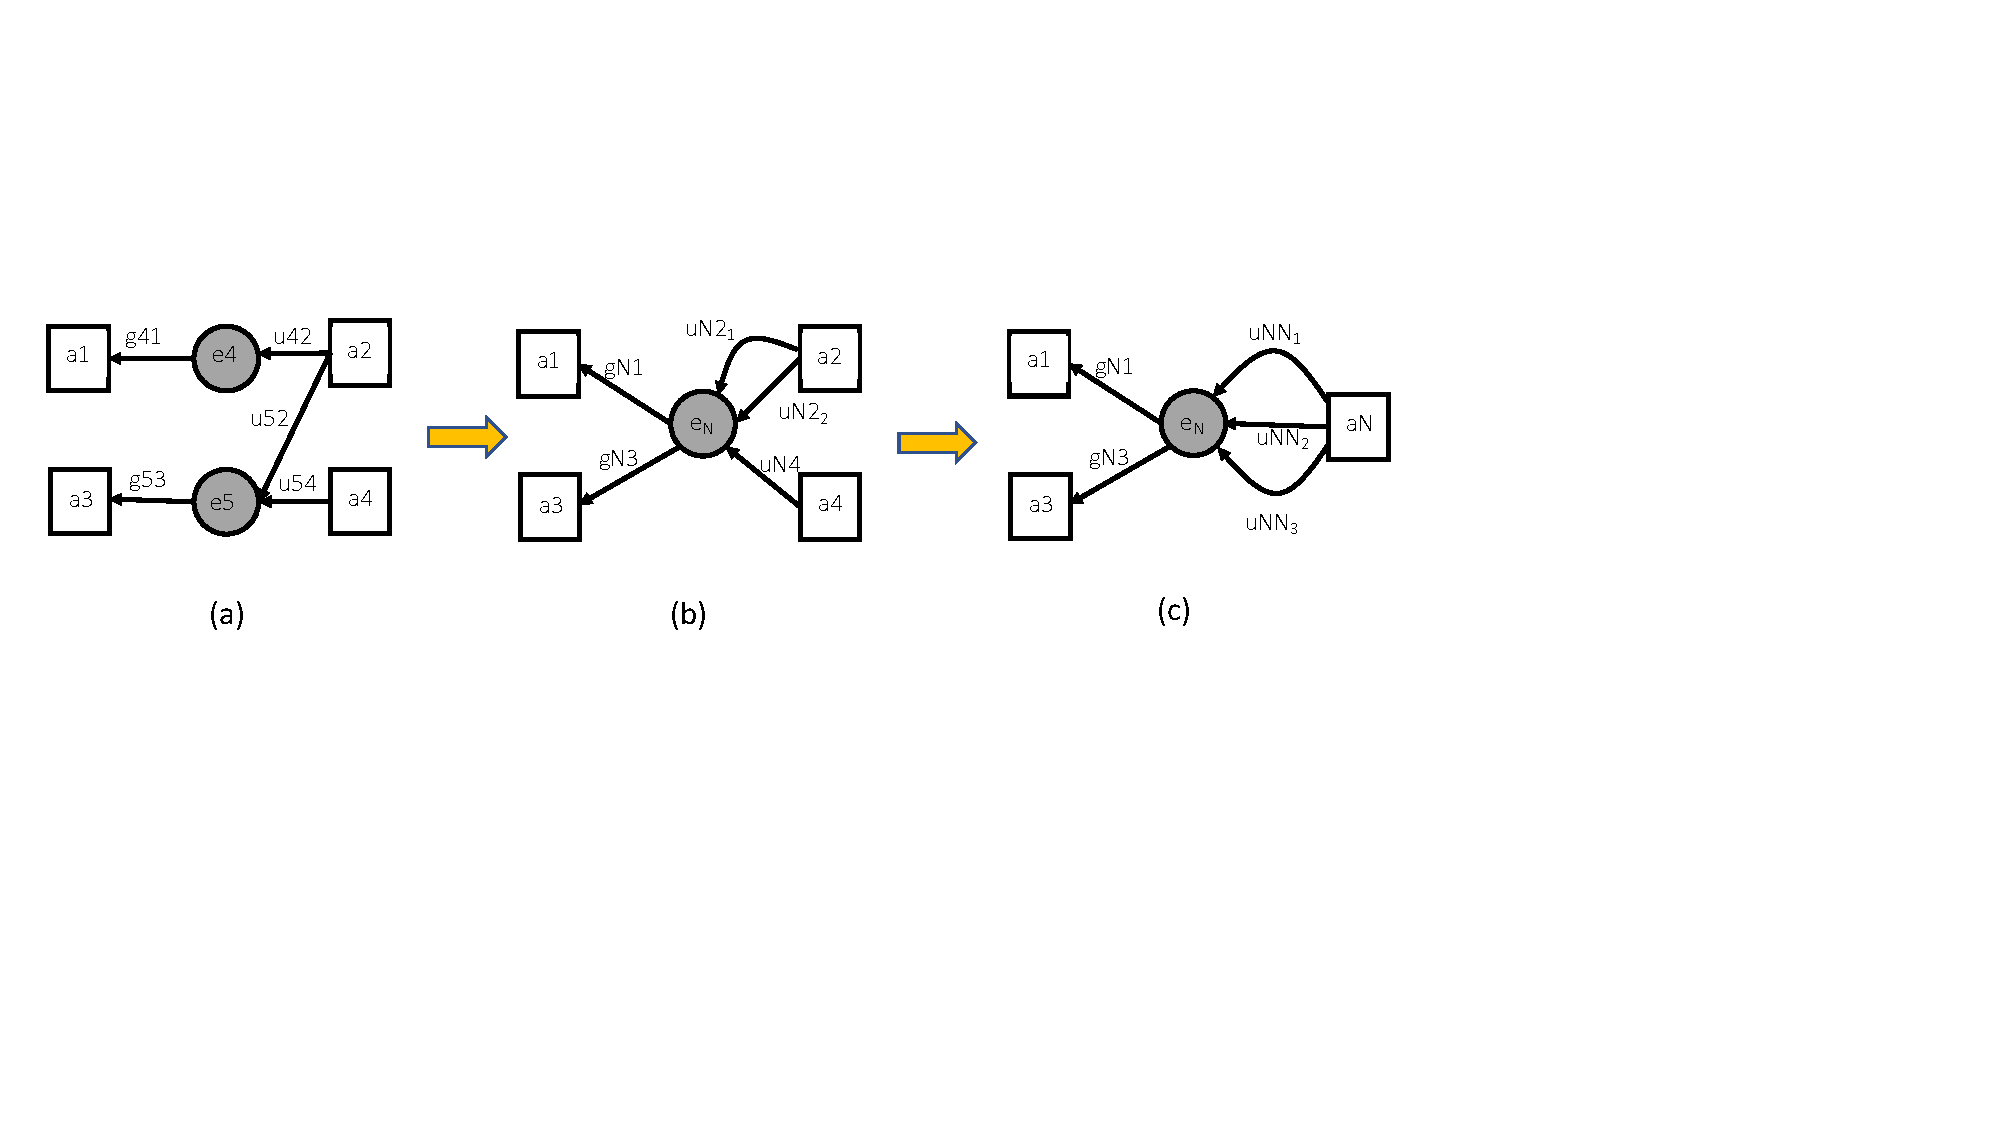
\includegraphics[scale=.5]{cropped-reworked-e4-e5.pdf} 
	\caption{Abstraction over a document content, and associated abstracted events} \label{fig:e4-e5}
\end{figure*}

In Sec.~\ref{sec:prov-constraints} we recalled the definition of PROV ordering  constraints C2-C7, given in the PROV-CONSTRAINT document, which must be satisfied by any valid PROV graph.
We now want to extend such formal definition of validity to include \textit{abstract} graphs $G^{A}$. 
To achieve this, we must first define suitable events on $G^{A}$. 
When $G^{A}$ is obtained using either e-grouping or a-grouping over some \jwbtwo{concrete} base graph $G^{C}$,  in general these are not the same events as $G^{C}$'s, because both entities and relationships may have changed. 
Specifically, when $a_{new}$ is created through a-grouping, $G^{A}$s events include 
 $start(a_{new})$, $end(a_{new})$, as well as 
$ev(\used(e, a_{new}))$, $ev(\wgby(a_{new}, e))$ for all $e$ that are generated by or used by $a_{new}$. 
For e-grouping, the new events are $ev(\wgby(e_{new}, a))$ and  $ev(\used(e_{new},a))$ for any $a$ that has generated (resp. used) $e_{new}$.
%
We are going to refer to the two sets of events in $G^{C}$ and $G^{A}$ as $EV_{G^{C}}$, $EV_{G^{A}}$, respectively.

Note: we use symbols such as $g_{41}$ in the figure to indicate relationships like $\wgby(e_4, a_1)$. 
With slight abuse of notation, but in the interest of simplicity, in the following we are going to use $g_{41}$ to also denote $ev(\wgby(e_4, a_1))$ when it is clear from the context that we refer to the event rather than to the relationship itself.

To fix ideas, consider $G^{C}$ in Fig.~\ref{fig:e4-e5}(a), where two sections of a document are independently generated by two editing activities, and then they are independently used by four more activities. Note that this is a slight extension of the abstract pattern of Fig.~\ref{fig:e2-a4}, where the document sections are $e_4$, $e_5$.
%
The e-grouping set $V_{gr} = \{ e_4, e_5\}$ represents the whole document. 

Let $G^{A}$ be the result of (non-strict) e-grouping, as depicted in Fig.~\ref{fig:e4-e5}(b), where the abstract generation and usage events are given new names, namely $g_{Ni}$ as a shorthand for $\wgby(e_N,a_i)$, and $u_{Ni_j}$ for each usage $j$ of the form $\used(a_i, e_N)$. 
Thus, $EV_{G^{C}} = \{ g_{41}, g_{53}, u_{42}, u_{52}, u_{54} \}$ and $EV_{G^{A}} = \{ g_{N1}, g_{N3}, u_{N2_1}, u_{N2_2}, u_{N4} \}$.
%
If $G^{C}$ is valid, the following must hold (constraint C3):
\begin{align}
\label{eq:c3-G}
g_{41} \preorder u_{42}, \quad g_{53} \preorder u_{52}, \quad g_{53} \preorder u_{54} 
\end{align}
where $\preorder$ is the preorder relationship introduced in Section~\ref{sec:prov-events}.

Similarly, for $G^{A}$ to be valid we must have:
\begin{align}
g_{N1} \preorder u_{N2_1}, \quad g_{N1} \preorder u_{N2_2}, \quad g_{N1} \preorder u_{N4}  \label{eq:c3-global1} \\  
g_{N3} \preorder u_{N2_1}, \quad g_{N3} \preorder u_{N2_2}, \quad g_{N3} \preorder u_{N4} \label{eq:c3-global2} 
\end{align}

Recall that the PROV-DM recommendation document~\citep{w3c-prov-dm} defines generation and usage events as follows:
%\begin{description}
\begin{itemize}
	\item\textbf{Generation} \textit{is the completion of production of a new entity by an activity} (Sec. 5.1.3 of~\citep{w3c-prov-dm})
	\item\textbf{Usage} \textit{is the beginning of utilizing an entity by an activity} (Sec. 5.1.4 of~\citep{w3c-prov-dm})
%	\item\textbf{Invalidation} \textit{is the start of the destruction, cessation, or expiry of an existing entity by an activity. The entity is no longer available for use (or further invalidation) after invalidation. Any generation or usage of an entity precedes its invalidation.} (Sec. 5.1.8)
\end{itemize}

Thus, $e_{N}$ is generated when both generation events $g_{N1}, g_{N3}$ have occurred (incidentally, this implies that these abstract events must be simultaneous), and it starts being used when the ``earliest'' of the usage events takes place, keeping in mind that no ordering relationships amongst the usage events is necessarily defined.

Intuitively, it should be possible to map abstract events to corresponding  original events in $G^{C}$, in such a way that validity of $G^{A}$ follows from the validity of $G^{C}$.
%
To formalise this idea, we propose to define the  events in $EV_{G^{A}}$ in terms of events in $EV_{G^{C}}$, that is, by means of a function $\psi$ that maps each $ev^{A} \in EV_{G^{A}}$ to a corresponding event in $EV_{G^{C}}$:
\begin{align}
 \psi: EV_{G^{A}} \rightarrow EV_{G^{C}} 
\end{align}
Furthermore, we want $\psi$ to be order-preserving, so that the validity of $G^{A}$ relative to temporal constraints can be derived from the validity of $G^{C}$ using $\psi$, \jwbtwo{
so if $s_1$ and $s_2$ are events: 
\begin{align}
 s_1 \preorder s_2 \Rightarrow \psi(s_1) \preorder \psi(s_2)  
\end{align}
}
where the same preorder $\preorder$ is used for both sets (because that is defined by the constraints).

We now look for a suitable mapping $\psi$. Consider for instance:
\begin{equation}
\psi(g_{N1}) = g_{41} ,  \quad  \psi(g_{N3}) =  g_{53},  \quad   \psi(u_{N2_1}) = u_{42}  \quad \psi(u_{N2_2}) = u_{52} \quad \psi(u_{N4}) = u_{54} \label{eq:psi-zero}
\end{equation}
This is a ``natural'' mapping, which follows the mapping between abstract and original relationships induced by the grouping operator.
Since $\psi$ is order-preserving, from (\ref{eq:psi-zero}) and (\ref{eq:c3-global2}), it follows that:
\begin{equation}
  g_{41} \preorder   u_{52}, \quad  g_{53} \preorder   u_{42}
  \label{eq:over-constraints-1}
  \end{equation}
However, we observe that neither of these relationships hold on $EV_G$, in fact the ordering of $g_{41}$ (resp $g_{53}$) relative to $u_{52}$ (resp $u_{42}$) is undefined.
Thus, if we consider all the possible total orderings in $EV_G$ that are consistent with $\preorder$, we see that this choice of mapping function restricts the possible interpretations of $EV_{G^{A}}$, when we assume that $G^{A}$ is valid, to only a subset of these orderings, namely those where the additional relationships (\ref{eq:over-constraints-1}) also hold.

We use this example to motivate a broader definition of $\psi$ that does not incur such restriction. For this, we first redefine $\psi$ to map each event in $EV_{G^{A}}$ to a \textit{set} of events in $EV_{G^{C}}$:
\begin{align}
 \psi': EV_{G^{A}} \rightarrow {\cal P}(EV_{G^{C}}) 
\end{align}
(where ${\cal P}(EV_{G^{C}})$ denotes a powerset \jwbtwo{of concrete events}).
%
Then, we introduce a new preorder $\preorderprime$  on ${\cal P}(EV_{G^{C}})$, such that
\jwbtwo{if $S_1, S_2$ are sets of events, and $s_1, s_2$ events, then}:
\begin{align}
 S_1 \preorderprime S_2 \text{ iff for each } s_1 \in S_1, \exists s_2 \in S_2 \text{ such that } s_1 \preorder s_2 
 \end{align}
We can now define \jwbtwo{a new} mapping $\psi'$ that is order-preserving:
\jwbtwo{
\begin{align} 
s_1 \preorder s_2 \Rightarrow \psi(s_1) \preorderprime \psi(s_2)  
%ev_1' \preorder ev_2' \Rightarrow \psi(ev_1') \preorderprime \psi(ev_2')  
\end{align}
}
as follows:
\jwbtwo{
\begin{equation}
\psi'(g_{N1}) = \{ g_{41}, g_{53} \},  \quad  \psi'(u_{N2_1}) =  \psi'(u_{N2_2}) = \{ u_{42}, u_{52} \}, \quad \psi'(u_{N4}) = \{u_{54} \} \label{eq:psi-real}
%\psi(g_{N1}) = \{ g_{41}, g_{53} \},  \quad  \psi(u_{N2_1}) =  \psi(u_{N2_4}) = \{ u_{42}, u_{52} \}, \quad \psi(u_{N4}) = \{u_{54} \} \label{eq:psi-real}
\end{equation}
}
It is easy to see for example that, with this mapping, the constraints 
$g_{N1} \preorder u_{N2_1}$, $g_{N3} \preorder u_{N2_2}$ both imply $ \{ g_{41}, g_{53} \} \preorderprime  \{ u_{42}, u_{52} \} $,
which includes interpretations on $G^{C}$ where the new constraints (\ref{eq:over-constraints-1}) need not hold.
The specification of $\psi'$ follows easily from the computation of the grouping operator, and details are omitted.

In summary, we have proposed to introduce (i) a set of abstract events on $G^{A}$ so we can verify its validity relative to temporal constraints, (ii) a mapping function that defines abstract events in terms of original events in $G^{C}$, and (iii) a set-based preorder such that the mapping can be order-preserving without imposing additional constraints on $G^{C}$. 


%%OBSOLETE. retrieve from git is we change our minds.
%\subsection{Mappings for abstract events }
%
%The following questions provide a useful starting point for reasoning about events. Firstly, given the generation events $g_{41}$, $g_{53}$  of each of the document sections, when was the entire document $e_N$ generated? 
%%
%When did $a_2, a_4$ use the document? 
%%
%Secondly,  suppose after the first grouping one performs two additional a-groupings, first with $V_{gr} = \{a_1, a_3\}$, and then with $V_{gr} = \{a_2, a_4, a_5, a_6\}$.
%%
% This results in the abstraction depicted in Fig.~\ref{fig:e4-e5}(c), which reads simply ``(abstract) document $e_N$ was used by (abstract) activity $a_N$''. 
% In this abstraction, what happens to the original generation and usage events?
%
%Initial help in answering these questions comes from the PROV-DM recommendation document~\citep{w3c-prov-dm}, namely:
%%\begin{description}
%\begin{itemize}
%\item\textbf{Generation} \textit{is the completion of production of a new entity by an activity} (Sec. 5.1.3)
%\item\textbf{Usage} \textit{is the beginning of utilizing an entity by an activity} (Sec. 5.1.4)
%\item\textbf{Invalidation} \textit{is the start of the destruction, cessation, or expiry of an existing entity by an activity. The entity is no longer available for use (or further invalidation) after invalidation. Any generation or usage of an entity precedes its invalidation.} (Sec. 5.1.8)
%\end{itemize}
%%\end{description}
%
%%
%Let us consider these definitions in the context of our example. Firstly, the generation of the whole document is only complete upon generation of the last section. Thus, each of the generation events of $e_N$, denoted $g_{N1}$ and $g_{N3}$ in Fig.~\ref{fig:e4-e5}(b), cannot precede $g_{41}$, $g_{53}$. This can be written as the ordering constraints:
%\begin{align}
% \label{eq:gprime-order1}
%max\{g_{41}, g_{53}\} \leq g_{N1} \\
%max\{g_{41}, g_{53}\}  \leq g_{N3}
%\end{align}
%Furthermore, we know from constraint C2 that $g_{N1}$ and $g_{N3}$ must be simultaneous:
%$g_{N1} = g_{N3}$.
%
%
%Secondly, symmetrically to generation, usage of the document ($u_{N2_1}, u_{N2_2}, u_{N4}$) in Fig.~\ref{fig:e4-e5}(b) begins with the earliest usage by any of the consuming activities:
%\begin{align}
%u_{N2_1} \leq u_{42} \label{eq:gen-usage1}\\
%u_{N2_2} \leq u_{52}  \label{eq:gen-usage2}\\
%u_{N4} \leq u_{54}  \label{eq:gen-usage3}
%\end{align}
%%
%Finally, from the definition above, the rule for invalidation follows the same pattern as usage:
%%
%\begin{align}
%i_{N6} &\leq i_{46} \label{eq:inv1}\\
%i_{N5} &\leq i_{55}  \label{eq:inv2}
%\end{align}
%%
%Furthermore, C3 requires each generation to precede each usage:
%%
%\begin{align}
%g_{N1} &= g_{N13}  \leq  u_{N2_1}  \quad  \\
%g_{N1} &= g_{N13}  \leq  u_{N2_2}  \quad  \\
%g_{N1} &= g_{N13}  \leq  u_{N4}  \label{eq:gprime-order2}
%\end{align}
%%
%and C4, C5 require both generation and usage to precede invalidation:
%%
%\begin{align}
%g_{N1} &= g_{N3} \leq i_{N6}  \quad g_{N1} = g_{N3} \leq i_{N5} \\
%u_{N2_1} &\leq i_{N6}  \quad u_{N2_1} \leq i_{N5} \\
%u_{N2_2} &\leq i_{N6}  \quad u_{N2_2} \leq i_{N5} \label{eq:inv-last}
%\end{align}
%%
%In order to avoid excessive clutter in the example, start and generation constraints are only discussed in the next section, along with all general ordering constraints on $G'$.
%
%
%Now, consider the  linear orderings in $G$ under the assumption that \textit{every generation event precedes every usage event} and \textit{every usage event precedes every invalidation event}, that is, there is a ``generation phase'' followed by a ``usage phase'' and by an ``invalidation phase'' (Fig.~\ref{fig:e-grouping-orderings}(a)). It is easy to see that, with this assumption, all these orderings are consistent with constraints (\ref{eq:gprime-order1}) through (\ref{eq:inv-last}), provided that we redefine $G'$ events to be \textit{simultaneous} to corresponding $G$ events, as follows:
%
%\begin{figure*}
%\centering
%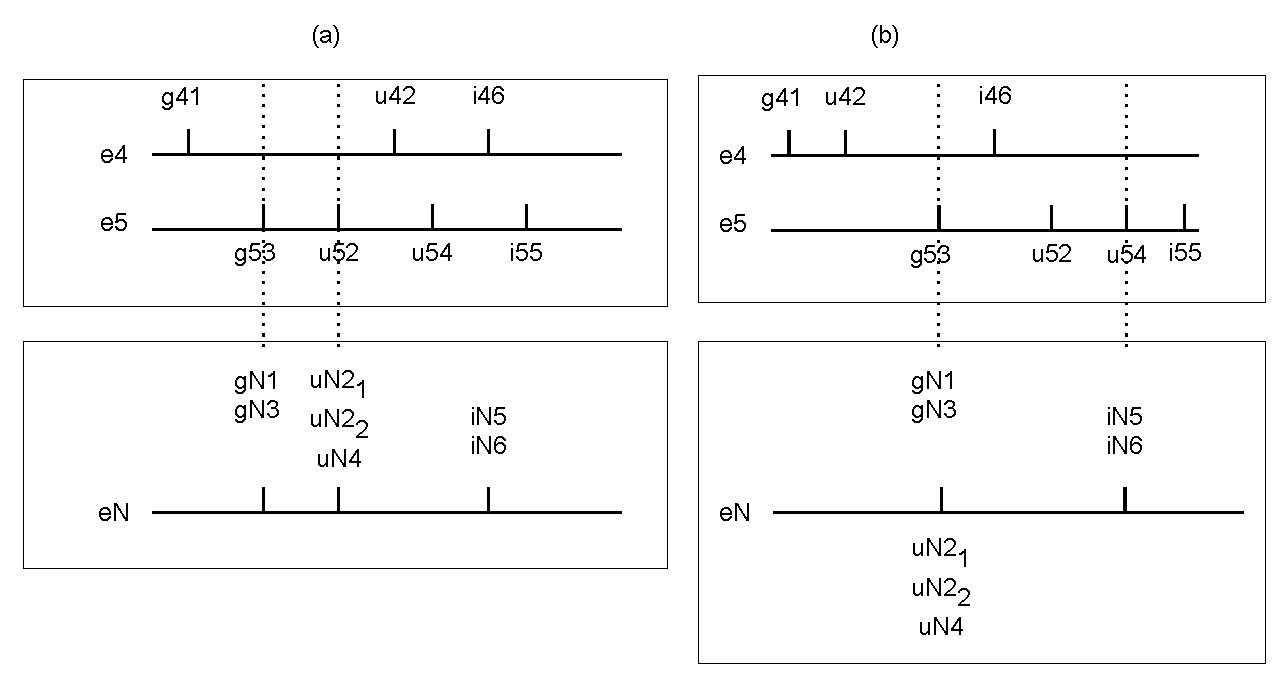
\includegraphics[scale=.5]{figures/e-grouping-orderings.pdf} 
%\caption{Two possible orderings on $G$ (top), and corresponding orderings on $G'$ (bottom)} \label{fig:e-grouping-orderings}
%\end{figure*}
%
%
%\begin{align}
%g_{N1} = g_{N3} = max\{g_{41}, g_{53}\}   \label{eq:max} \\
%u_{N2_1} = u_{N2_2}  = u_{N4} = min\{u_{42},  u_{52},  u_{54}\}   \label{eq:usage-min-simple} \\
%i_{N5} = i_{N6}  = min \{   i_{46},  i_{55} \}   \label{eq:inval-min-simple}
%\end{align}
%In this case we conclude that $G'$ is valid by our assumption that each of its generation events precedes each of its usage events.
%
%Consider now the more general case where generation, usage and invalidation events are interleaved for different entities in $V_{gr}$. Fig.~\ref{fig:e-grouping-orderings}(b) shows such an interleaving for our example. In this case, 
%$min \{   u_{42},  u_{52},  u_{54} \} = u_{42} \leq g_{53} = max\{g_{41}, g_{53}\}$.
%%
%This violates (\ref{eq:gen-usage1}) through (\ref{eq:gen-usage3}).  In other words, this more general family of interpretations over $G$ is not represented in $G'$ when the abstract events in $G'$ are defined using the inequalities above. 
%
%In order to account for this general case, we modify  (\ref{eq:usage-min-simple}) and (\ref{eq:inval-min-simple}) as follows:
%\begin{align}
%u_{N2_1} &= u_{N2_2}  = u_{N4} = max\{ g_{41}, g_{53}, min \{u_{42},  u_{52},  u_{54}\}\}  \label{eq:usage-min} \\
%i_{N5} &= i_{N6}  = max\{g_{41}, g_{53}, u_{42},  u_{52},  u_{54}, min\{i_{46},  i_{55}\}\}   \label{eq:inval-min}
%\end{align}
%%
%
%In the example of Fig.~\ref{fig:e-grouping-orderings}(b), this stricter constraint results in  generation and usage events in $G'$ to all be simultaneous to $g_{53}$, while the invalidation events are shifted later in the event line, to the latest usage. Note that in the special case of Fig.~\ref{fig:e-grouping-orderings} (a), constraints (\ref{eq:usage-min-simple}), (\ref{eq:usage-min}) and (\ref{eq:inval-min-simple}), (\ref{eq:inval-min})  are pairwise equivalent.
%
%The reasoning used in the examples just presented justifies the following definitions for the general inequalities which define abstract events in terms of events in $G$.
%
%\subsection{Abstract events for e-grouping}
%\label{sec:abstract-events-for-e-grouping}
%%
%Let $G=(V,E) \in \guEA$, $V_{gr} \subset V$ be the set of nodes that are to be grouped, and  $e_{new} \in \en$ be the new entity node introduced through e-grouping as per Def.~\ref{eq:t-grouping}.
%% 
%
%\paragraph*{\textbf{Abstract Generation events}}
%Let $V^*$ to denote $\extend(\clos(V_{gr},G), \en)$, and let $\wgby_{out}$ denote the set of generation relations involving entity nodes in the extension
%$V^*$, and activity nodes outside of the extension:
%\begin{align*} 
%\wgby_{out} = \{ \wgby(e,a) |  e \in V^*,  a \notin V^* \}
%\end{align*} 
%In the example of Fig.~\ref{fig:e4-e5}, $\wgby_{out} = \{ g_{41}, g_{53} \}$.
%
%%
%Correspondingly, let $\wgby'_{out}$ denote the generation relations that involve $e_{new}$:
%\begin{align*} 
%\wgby'_{out} = \{ \wgby(e_{new},a) | a \notin V^* \}
%\end{align*} 
%In the example, $\wgby'_{out} = \{ g_{N1}, g_{N3} \}$.
%
%In general, we will denote values in the abstracted prov graph by primed versions of their counterparts in the original graph. The exception to this will be relationships and events involving $e_{new}$, since $e_{new}$ is  a new entity that does not appear in the old graph.
%
%The following equalities, define the orderings of the events associated with the relations in $\wgby'_{out}$.
%
%
%\vspace*{10pt}
%\begin{definition}[Abstract generation events - e-grouping]
%\label{def:abstract-gen-e}
%
%\paolotwo{Replace max with a new event that dominates all of the $ev(g)$ and adjust the def below accordingly}
%
%For each $g' \in \wgby'_{out}$:
%\[
%ev(g') = max \{ ev(g) | g \in \wgby_{out} \}  
%\]
%For all activities $a$ that participate in generating the new event $e_{new}$, we set the generation event to
%\[
%ev(\wgby(e_{new},a)) = max \{ ev(g) | g \in \wgby_{out} \}
%\]
%\end{definition}
%
%%\vspace*{10pt}
%%\begin{definition}[Abstract usage events - e-grouping] 
%%\label{def:abstract-usage-e}
%%Let
%%\[u'_{min} = min_{ u \in \used_{in} } ( ev(u) \}\] and let 
%%$g'_{max} = max_{g \in \wgby_{out}} ( ev(g) \} $.\\
%%For each $u' \in \used'_{in}$:
%%\begin{equation}
%%v(u') = max \{ g'_{max} , u'_{min} \}
%%\end{equation}
%%\end{definition}
%
%\paragraph*{\textbf{Abstract Usage events}}
%Usage events for e-grouping are defined similarly by generalization from (\ref{eq:usage-min}), as follows.
%%
%Let $\used_{in}$ denote the set of usage relations involving entity nodes in the extension
%$V^*$, and activity nodes outside of the extension:
%\begin{align*} 
%\used_{in} = \{ \used(a,e) |  e \in V^*,  a \notin V^* \}
%\end{align*} 
%In the example of Fig.~\ref{fig:e4-e5}, $\used_{in} = \{ u_{42}, u_{52}, u_{54} \}$.
%
%%
%Correspondingly, let 
%$\used'_{in}$ denote the usage relations that involve $e_{new}$:
%\begin{align*} 
%\used'_{in} = \{ \used(a, e_{new}) | a \notin V^* \}
%\end{align*} 
%In the example, $\used'_{in} = \{ u_{N2_1}, u_{N2_2}, u_{N4}  \}$.
%
%The following equalities, which generalise (15), define the events associated with the relations in $\used'_{in}$.
%
%\vspace*{10pt}
%\begin{definition}[Abstract usage events - e-grouping] 
%\label{def:abstract-usage-e}
%
%
%\paolotwo{min does not always exist so as for max, we need to introduce a new $u$ that is $\leq$ than all of the usage events, and adjust the def below accordingly}
%Let
%\[u'_{min} = min \{ ev(u) | u \in \used_{in} \}\] and let 
%$g'_{max} = max \{ ev(g) | g \in \wgby_{out}\} $.\\
%For each $u' \in \used'_{in}$:
%\begin{equation*}
%ev(u') = max \{ g'_{max} , u'_{min} \}
%\end{equation*}
%and so
%\begin{equation}
%ev(\used(a,e_{new})) = max \{ g'_{max} , u'_{min} \}
%\end{equation}
%\end{definition}
%
%\paolotwo{remove invalidation altogether}
%\paragraph*{\textbf{Abstract Invalidation events}}
%The events equalities for invalidation, exemplified in (\ref{eq:inval-min}), follow the pattern used above for usage. The only difference is that $\used'_{in}$ is replaced by 
%\[ \inv'_{in} = \{ \inv(a, e_{new}) | a \notin V^* \} \]
%In our example, $ \inv_{in} = (  i_{46}, i_{55} \}$,  $\inv'_{in} = ( i_{N6}, i_{N5} \}$.
%%
%The corresponding definition is as follows.
%
%\vspace*{10pt}
%\begin{definition}[Abstract invalidation events] 
%\label{def:abstract-inv}
%Let
%\[i'_{min} = min \{ ev(i) | i \in \inv_{in} \}\]
%and 
%\[u'_{max} = max \{ ev(u) | u \in \used_{in} \}\]
%For each $i' \in \inv'_{in}$:
%\[
%ev(i') = max \{ g'_{max} , u'_{max},  i'_{min}\}
%\]
%and thus for each activity $a$  that participates in the invalidation of $e_{new}$, invalidation is the latest of the new generation event $g'_{max}$, the latest usage event $u'_{max}$ and the minimum of the original invalidation events.  
%\begin{equation}
%\inv(a,e_{new}) = max \{ g'_{max} , u'_{max},  i'_{min} \}
%\end{equation}
%\end{definition}
%
%
%{\bf Start events:} Now that the event of usage and generation of $e_{new}$ has been fixed, we need to ensure that the activities involved in these events continue to meet the constraints that apply to them. This includes start and end events for activities related to our new entity $e_{new}$ by either $\wgby$ or $\used$.  
%
%
%%In addition, a-grouping also produces new abstract start and end events for the new activity $a_{new}$. 
%% The situation is illustrated in the timelines of Fig.~\ref{fig:a1-a2}. The right side of figure (a) shows a possible interleaving of events in $G$, which is consistent with constraints C2-C7. Intuitively, the start (resp. end) event for the abstract activity $a_N$ cannot follow (resp. precede) the earliest (resp., latest) usage/generation event associated with $a_1, a_2$.
%% %
%% Similar to the case for e-grouping,
%We appeal to the informal definitions of start and end in~\citep{w3c-prov-dm} to derive inequalities for the abstract start and end events for our new activity $a_{new}$.
%% 
%\begin{itemize}
%\item \textbf{Start} \textit{is when an activity is deemed to have been started by an entity, known as trigger. The activity did not exist before its start. Any usage, generation, or invalidation involving an activity follows the activity's start} (See~\citep{w3c-prov-dm},  Section 5.1.6)
%
%\item \textbf{End} \textit{is when an activity is deemed to have been ended by an entity, known as trigger. The activity no longer exists after its end. Any usage, generation, or invalidation involving an activity precedes the activity's end} (See~\citep{w3c-prov-dm}, Section 5.1.7)
%\end{itemize}
%(For simplicity we are going to leave the trigger entity implicit, and simply refer to the start and end events as $\start(a)$ and $\ed(a)$).
%
%\paolotwo{do not think we need (27) because it is implied by the mapping for the abstract generation events. probably (28) not needed either }
%\begin{definition}[Start events - e-grouping] 
%\label{def:abstract-start-e}
%Consider events $a$ such that $\wgby(e_{new},a)$. For each such $a$, we set the new start event $\start'(a)$ as the lesser of the original start event and the generation event $ev(\wgby(e_{new},a))$. Thus
%\begin{equation}
%\start'(a) = min\{\start(a),ev(\wgby(e_{new},a))\}
%\end{equation}
%\end{definition}
%
%{\bf End events:} For all activities $a$ that use the newly created entity, we must ensure that ensure that the end of the activity does not precede any $\used(a,e_{new})$ events.
%\begin{definition}[End events - e-grouping]
%  \label{def:abstract-end-e}
%  If the set of all usage events by $a$ of $e_{new}$ is denoted $\{ev(\used(a,e_{new}))\}$, we set the new end events $\ed'(a)$ to be
%  \begin{equation}
%  \ed'(a) = max\{\ed(a), max\{ev(\used(a,e_{new}))\}\}
%\end{equation}
%\end{definition}
%
%A proof of that, given the definitions above, the  constraints of Section~\ref{sec:prov-constraints} are satisfiable, is given in~\ref{sec:consistency-constraints-e-grouping}.
%
%
%\subsection{Abstract events for a-grouping}
%\label{sec:abstract-events-for-a-grouping}
%% \begin{figure}
%% \centering
%% 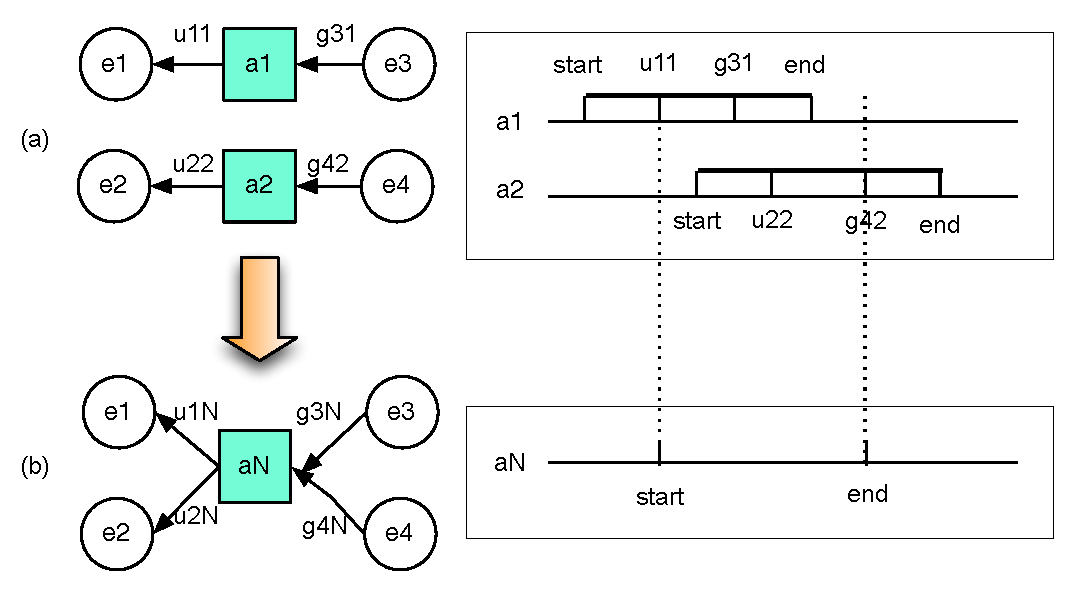
\includegraphics[scale=.5]{figures/a1-a2.pdf} 
%% \caption{Abstraction for start/end events} \label{fig:a1-a2}
%% \end{figure}
%
%Generation and usage abstract events follow a very similar pattern as those for e-grouping, except that the new node introduced by grouping is an activity node: $a_{new} \in \act$.
%%
%%This is illustrated in Fig.~\ref{fig:a1-a2}.
%As a consequence, the abstract event definitions given in the previous section also follow the same pattern, but with the roles of entities and activities reversed. They are summarized here below.  We now use $V^*$ to mean the group of nodes collected by $\extend(\clos(V_{gr},G), \act)$.
%
%%\jwb{I (personally) find the notations below confusing, and would rather get rid of them. I haven't used them much in the rest of this section.}
%%
%%\begin{align*} 
%%\wgby_{in} & =  \{ \wgby(e,a) |  e \notin V^*, a \in V^* \} \\
%%\wgby'_{in} &  = \{ \wgby(e, a_{new}) | e \notin V^* \} \\
%%\used_{out} & = \{ \used(a,e) |  e \notin V^*,  a \in V^* \} \\
%%\used'_{out} & = \{ \used(a_{new}, e) | e \notin V^* \}
%%\end{align*} 
%%
%%
%%
%
%\paolotwo{def 14 makes no sense as we again need to introduce artificial min and max to account for the abstract start and end events}
%The new start (resp. end) event is taken to be the minimum (resp. maximum) relevant start (resp. end)  event.
%\begin{definition}[Abstract start and end events - a-grouping] 
%\label{def:abstract-start-and-end-a}
%\begin{align*}
%  \start(a_{new}) & = min\{\start(a) | a \in V^*\} \\
%  \ed(a_{new}) & = max\{\ed(a) | a \in V^*\} \\
%\end{align*}
%\end{definition}
%
%\begin{definition}[Abstract generation events - a-grouping]
%\label{def:abstract-gen-a}
%%Since generation events must be simultaneous, we can assume that they are simultaneous in the original graph. 
%%
%%For any entity $e$ not in $V^*$ that is generated by an activity $a$ in $V^*$, the new generation event cannot be before the start of the abstracted activity $a_{new}$, taken as the minimum of the original start events s in Definition~\ref{def:abstract-start-and-end-a}. However,
%Constraint C2 applies to the original graph, so for all activities $a,b$ that participate in the generation of $e$, $ev(\wgby(e,a)) = ev(\wgby(e,b))$. 
%
%
%%\jwb{Should we do start and end definitions first? Start and end only apply to ctivities, so the definition below already excludes entities}
%The new generation event is thus given as
%%  \begin{align*}
%%   ev(\wgby(e,a_{new})) =  max\{ &  \start(a_{new}), \\ 
%%                                & min\{ev(\wgby(e,a))  | a \in V^*\} \}
%% \end{align*}
%  \begin{align*}
%   ev(\wgby(e,a_{new})) =  ev(\wgby(e,a))
% \end{align*}
%
%\end{definition}
%
%\vspace*{10pt}
%\begin{definition}[Abstract usage events - a-grouping] 
%\label{def:abstract-usage-a}
%For an entity $e$ not in $V^*$ which is used by an activity $a$ in $V^*$, the assigned usage event for $a_{new}$ ($ev(\used(a_{new},e))$) is given by  
%\begin{align*}
%ev(\used(a_{new},e)) = max\{ & \start(a_{new}) , \\
%                            & min\{ev(\used(a,e))) | a \in V^*\}\}
%\end{align*}
%\end{definition}
%
%
%\vspace*{10pt}
%\begin{definition}[Abstract invalidation events - a-grouping] 
%  \label{def:abstract-inv-a}
%  By Constraint C8, invalidation events from two distinct activities are simultaneous.
% %
%For an entity $e$ which is invalidated by an activity $a$ in $V^*$, the event of the invalidation event remains the same when the activity is abstracted.
%\[
%ev(\inv(a_{new},e)) = min\{ev(\inv(a,e)) | a \in V^*\}
%\]
%\end{definition}
%
%A proof of that, given the definitions above, the  constraints of Section~\ref{sec:prov-constraints} are satisfiable, is given in~\ref{sec:consistency-constraints-e-grouping}.


